\documentclass[12pt,oneside]{article}
\usepackage{light}
\newcommand{\mfigure}[3]{\bigskip\centerline{\resizebox{#1}{#2}{\includegraphics{#3}}}\bigskip}

%\showsolutions
\hidesolutions


\begin{document}
\generic{Quiz 1}{October 18, 2006}



\instatements{

\textbf{Circle the name of your recitation instructor}:

\begin{center}
\begin{tabular}{lllllll}
Bill & Brooke & Chieu & Jay & Ling & Nick & Spyros 
\end{tabular}
\end{center}

\begin{itemize}

\item This quiz is \textbf{closed book}, but you may have one $8.5
\times 11$'' sheet with notes in your own handwriting on both sides.

\item Calculators are not allowed.

\item You may assume all of the results presented in class.

\item Write your solutions in the space provided.  If you
need more space, write on the back of the sheet containing the
problem.  Please keep your entire answer to a problem on that
problem's page.

\item Be neat and write legibly.  You will be graded not only on the
correctness of your answers, but also on the clarity with which you
express them.

\item If you get stuck on a problem, move on to others. The problems 
are not arranged in order of difficulty.

\item The exam ends at 9:00 PM.

\item For this quiz, $\mathbb N$ is the set of nonnegative integers 
(including 0): $\mathbb N = \{0,1, \ldots, \}$.

\item GOOD LUCK!

\end{itemize}

\vspace{0.25in}

\begin{center}
{\large
\begin{tabular}{|c|c|c|c|}
\hline
Problem & Points & Grade & Grader \\ \hline \hline
1 & 10 & & \\ \hline
Total & 10 & & \\ \hline
\end{tabular}
}
\end{center}
}



%%%%%%%%%%%%%%%%%%%%%%%%%%%%%%%%%%%%%%%%%%%%%%%%%%%%%%%%%%%%%%%%%%%%%
% taken from: new problem
% comments: number theory, predicates
%
\instatements{\newpage}
\begin{problem}{10} For this problem, assume the domain of discourse
to be the \emph{positive} integers.

\bparts

\ppart{5} Find a counter example to show that
\begin{equation}\label{numthypred}
\forall x,y \; . \quad \left[ x \equiv y \pmod{\phi(n)} \right] 
  \implies \left[ m^x \equiv m^y \pmod{n} \right]
\end{equation}
is not a validity.

\solution{}

\ppart{5} Prove that \eqref{numthypred} holds if $\gcd(m,n)=1$.

\solution{
If $x \equiv y \pmod{\phi(n)}$ then there must exist a $k$ such 
that $k \phi(n) = y - x$ by the definitions of congruence and 
divides.  Since $\gcd(m,n)=1$ by assumption, Euler's Theorem 
implies that
\[
\left( m^{\phi(n)} \right)^k \equiv 1 \pmod{n}
\]
and consequently that
\[
m^{y-x} \equiv 1 \pmod{n}.
\]
Multiplying both sides by $m^x$ proves the claim.
}

\ppart{5} {\bf Extra Credit} Multiple choice: what are the 
\emph{least} restrictive conditions on $n$ for which 
\eqref{numthypred} holds $\forall m$? 

\begin{enumerate}[a.]

\item $\phi(n)$ does not divide $n$

\item $n$ is prime

\item $n$ is a product of unique primes

\item $\gcd(n,\phi(n))=1$

\item none of the above

\end{enumerate}

\solution{$n$ is a product of unique primes}

\eparts
\end{problem}

%%%%%%%%%%%%%%%%%%%%%%%%%%%%%%%%%%%%%%%%%%%%%%%%%%%%%%%%%%%%%%%%%%%%%
% taken from: new problem
% comments: number theory
%
\instatements{\newpage}
\begin{problem}{7} 

\bparts

\ppart{2} Prove that 13 has an inverse modulo 165.

\solution{$165= 3 \cdot 5 \cdot 11$ and 13 are relatively prime 
since they don't share any prime factors and so 
there exists and inverse of 13 modulo 165.
}

\ppart{5} Use Euler's Theorem to find numerical value for 
$x$ in the range $\{0,1,2,\ldots,164\}$ such that
%
\begin{equation}\label{mod165exn}
13^{78} \cdot x \equiv 42 \pmod{165}.
\end{equation}

\solution{$x=3$

Since $\gcd(13,165)=1$, Euler's theorem implies
that $13^{\phi(165)} \equiv 1 \pmod{165}$ where 
$\phi{165}=\phi(3)\phi(5)\phi(11)=(3-1)(5-1)(11-1)=80$.

Therefore, multiplying both sides of \eqref{mod165exn} by
$13^2 = 169 \equiv 4$,
\begin{align*}
13^{80} \cdot x & \equiv 13^2 \cdot 42\\
      1 \cdot x & \equiv 4 \cdot 42\\
              x & \equiv 168 \equiv 3
\end{align*}
where the modulus for each of the equivalences is 165.
}

\eparts
\end{problem}



%%%%%%%%%%%%%%%%%%%%%%%%%%%%%%%%%%%%%%%%%%%%%%%%%%%%%%%%%%%%%%%%%%%

\begin{problem}{20}
For $n\geq 1$, let $a_n$ be the largest odd divisor of $n$, and let $b_n = a_1+a_2+ \ldots +a_n$. 

\bparts

\ppart{2} Prove the proposition that $a_{2n+1}=2n+1$. 

\solution{
\begin{proof}
The largest odd divisor of an odd number is the odd number itself.
\end{proof}
}

\ppart{5} Prove the proposition that $a_{2n}=a_n$.

\solution{
\begin{proof} Let $d$ be the largest odd divisor of $2n$. Since $d$ is odd,
$d$ must divide $n$. So, $a_{2n}\leq a_n$. Since the largest odd divisor of $n$ also divides $2n$, $a_n\leq a_{2n}$. Combining both inequalities proves the
proposition.
%If a divisor $d$ of $2n$ does not divide $n$, then $2$ must divide $d$.
%The contrapositive states that if $d$ is an odd divisor of $2n$, then it
%divides $n$. So, the largest odd divisor of $2n$ is equal to the largest
%odd divisor of $n$. 
\end{proof}
}

\ppart{10} Prove the proposition that $b_n\geq (n^2+2)/3$. 

Hint: use strong induction and when you prove the inductive hypothesis for $n+1$, distinguish the two cases $n+1$ is even (that is, $n+1=2k$ with $k\geq 1$) and $n+1$ is odd (that is, $n+1=2k+1$ with $k\geq 1$).

\solution{
\begin{proof}
We use strong induction. Let $P(n)$, for $n\geq 1$, be the predicate $b_n\geq (n^2+2)/3$.

{\bf Base case:}  
$b_1=a_1=1\geq (1^2+2)/3$. 

{\bf Inductive step:} For the purposes of proving $P(n+1)$, assume $P(k)$ for
$1 \leq k \leq n$. So, we assume that $b_k\geq (k^2+2)/3$ is true for 
$1 \leq k \leq n$. 

We distinguish the two cases $n+1$ is even and $n+1$ is odd.

If $n+1 = 2k$ with $k\geq 1$, then
\begin{eqnarray*}
b_{n+1} &=& (a_1 + a_3 + \ldots + a_{2k-1}) + (a_2 + a_4 +\ldots +a_{2k}) \\
&=& 1 + 3+\ldots +(2k -1) + (a_1 + a_2 + \ldots +a_k) \\
&=& k^2 + b_k \\
&\geq &  k^2 + (k^2 + 2)/3 \mbox{ (by the inductive hypothesis)} \\
&=& ((2k)^2 + 2)/3 \\
&=& ((n+1)^2+2)/3.
\end{eqnarray*}

If instead $n+1 = 2k + 1$
with $k\geq 1$, then
\begin{eqnarray*}
b_{n+1} &=& (a_1 + a_3 +\ldots +a_{2k+1}) + (a_2 + a_4 +\ldots +a_{2k}) \\
&=& 1 + 3+\ldots +(2k + 1) + (a_1 + a_2 +\ldots +a_k) \\
&=& (k + 1)^2 + b_k \\
&\geq& (k + 1)^2 + (k^2 + 2)/3 \mbox{ (by the inductive hypothesis)} \\
&=& ((2k + 1)^2 + 2)/3 +(2k+2)/3 \\
&>& ((n+1)^2 + 2)/3.
\end{eqnarray*}

\end{proof}
}

\ppart{0} DISREGARD THIS PART? 
Determine for which $n$ the equality $b_n=(n^2+2)/3$ holds. 
You do not need to prove your answer.

\solution{
The previous derivations show that, for odd $n+1$, $b_{n+1}>((n+1)^2 + 2)/3$, and, for even $n+1=2k$, $b_{n+1}=((n+1)^2+2)/3$ if and only if $b_k=(k^2 + 2)/3$.
This leads us to believe 
$$P(n) = ``b_n=(n^2+2)/3 \leftrightarrow n \mbox{ is a power of } 2''$$
for $n\geq 1$. 

\begin{proof} We use strong induction.

{\bf Base case:}  
$b_1=1= (1^2+2)/3$ and $1=2^0$, so $P(1)$ is true.

{\bf Inductive step:}
For the purpose of proving $P(n+1)$,
 suppose that $P(k)$ is true for $1 \leq k \leq n$.
If $n+1$ is odd $b_{n+1}>((n+1)^2 + 2)/3$ and $P(n+1)$ holds.
If $n+1=2k$ is even with $k\geq 1$, then $b_{n+1}=((n+1)^2+2)/3$ if and only if $b_k=(k^2 + 2)/3$, that is, if and only if $k$ is a power of $2$ by the inductive hypothesis. This proves $P(n+1)$, that is, $b_{n+1}=((n+1)^2+2)/3$ if and only if $n+1$ is a power of $2$.
\end{proof}
}

\eparts

\end{problem}

%%%%%%%%%%%%%%%%%%%%%%%%%%%%%%%%%%%%%%%%%%%%%%%%%%%%%%%%%%%%%%%%%%%%%
% taken from: new problem
% comments: elementary graph theory
%
\begin{problem}{??}
Consider this graph representing the main campus buildings at MIT

\vspace{12pt}
\centerline{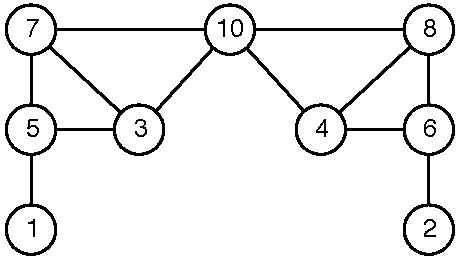
\includegraphics{maclaurin-graph}}
\vspace{12pt}

\bparts

\ppart{?} Give a maximum-length cycle in this graph:
\solution{3-7-10-5}

\ppart{?} Give a maximum-length path in this graph: 
\solution{1-3-5-7-10-6-8-4-2}

\ppart{?} Is this graph bipartite?
\solution{No, there is an odd-length cycle}

\ppart{?} Is the induced subgraph of nodes labeled by composite numbers complete?
\solution{No, there is no edge from 4 to 10}

\ppart{?} Draw a spanning tree of this graph:
\vspace {1in}
\solution{}

\ppart{?} Does this graph have an Euler circuit? Provide a brief argument for your answer (an example circuit is sufficient)
\solution{This graph does not have an Euler circuit because there are vertices with odd degree}

\ppart{?} Does this graph have a circuit that visits every edge exactly twice?
Provide a brief argument for your answer (an example circuit is sufficient)
\solution{}

\eparts
\end{problem}

%%%%%%%%%%%%%%%%%%%%%%%%%%%%%%%%%%%%%%%%%%%%%%%%%%%%%%%%%%%%%%%%%%%%%%%

\begin{problem}{15}
Define the sequence of numbers $A_i$, by

$A_0=2$ and

$A_{n+1}=A_n/2 + 1/A_n$, for $n\geq1$.

Prove that $A_n\leq \sqrt{2}+1/2^n$ for all $n\geq 0$. You may use the following result:

\begin{lemma*} For real numbers $x>0$, $x/2+1/x\geq \sqrt{2}$.
\end{lemma*}

\end{problem}

\solution{
\begin{proof}
We will use induction. For $n\geq 0$, 
let $P(n)$ be the predicate $A_n\leq \sqrt{2}+1/2^n$.

{\bf Base case:}  
$A_0=2\leq \sqrt{2}+1/2^0$ is true. 

{\bf Inductive step:}
Let $n\geq 0$ and suppose the inductive hypothesis $P(n)$, that is,
$A_n\leq \sqrt{2}+1/2^n$.
We need the following lemma.

\begin{lemma*} For real numbers $x>0$, $x/2+1/x\geq \sqrt{2}$.
\end{lemma*}

\begin{proof}
For real numbers $x>0$,
\begin{eqnarray*}
&& x/2+1/x\geq \sqrt{2} \\
&\leftrightarrow & x^2+2\geq 2\sqrt{2}\cdot x \\
&\leftrightarrow & x^2-2\sqrt{2} \cdot x+2 \geq 0 \\
&\leftrightarrow & (x-\sqrt{2})^2 \geq 0,
\end{eqnarray*}
which is true.
\end{proof}

 By using induction it is straightforward to prove that
$A_n>0$ for $n\geq 0$ (base case: $A_0=2>0$; inductive step: if $A_n>0$, then $A_{n+1}=A_n/2 + 1/A_n>0$). By the lemma,
$A_n\geq \sqrt{2}$ for $n\geq 0$.
Together with the induction hypothesis
this can be used in the following derivation:
\begin{eqnarray*}
A_{n+1} &=& A_n/2 + 1/A_n \\
&\leq & (\sqrt{2}+1/2^n)/2+1/\sqrt{2}\\
&=& \sqrt{2}+1/2^{n+1}.
\end{eqnarray*}

This completes the proof.
\end{proof}
}

%%%%%%%%%%%%%%%%%%%%%%%%%%%%%%%%%%%%%%%%%%%%%%%%%%%%%%%%%%%%%%%%%%%%%%%%

\begin{problem}{15}

An $n$-player \emph{tournament} consists of some set of $n\geq 2$
\emph{players}, and has the property that for every two players, $p \neq
q$, either $p$ beats $q$ or $q$ beats $p$, but not both.  
%\iffalse That is,
%player $p$ beats player $q$ iff $q$ does not beat $p$, for all players $p
%\neq q$.\fi

%A sequence of distinct players $p_1,p_2, \ldots, p_k$, such that each
%player beats the next one (that is, $p_i$ beats player $p_{i+1}$ for $1
%\leq i < k$) is called a {\em ranking} of these players.  

%If also player
%$p_k$ beats player $p_1$, the ranking is called a $k$-\emph{cycle}.

\begin{problemparts}

\ppart {10} Prove the proposition that if there exists a cycle of at least two nodes in the tournament graph, then there exists a cycle of three nodes.

\solution{Let $v_1\rightarrow v_2 \ldots \rightarrow v_h\rightarrow v_1$ be a smallest length cycle. Since the graph is a tournament, there do not exist cycles of length $2$. So, $h\geq 3$. If $v_1\rightarrow v_3$, then $v_1\rightarrow v_3\rightarrow v_4 \ldots \rightarrow v_h\rightarrow v_1$
is a shorter cycle of length $h-1$. This contradicts $h$ being the length of the shortest cycle. So, there is  no edge $v_1\rightarrow v_3$. Since the graph represents a tournament $v_3\rightarrow v_1$. So, $v_1\rightarrow v_2\rightarrow v_3\rightarrow v_1$ is
a cycle of length 3, therefore $h\leq 3$. So, $h=3$.
}

\ppart {5} A {\em consistent ranking} is a sequence $p_1,p_2, \ldots,
p_n$ of all $n$ players in the tournament such that each player beats all
the later players in the sequence (that is, $p_i$ beats $p_j$ iff $i < j$,
for $1 \leq i,j \leq n$). Prove by using the previous problem parts, that a tournament has no consistent ranking \textit{iff} some subset of three of its players has no consistent ranking.

\solution{
A tournament has no consistent ranking iff there exists a cycle.
There exists a cycle iff  
there exists a 3-cycle by part a. 
There exists a 3-cycle iff  some subset of three players has no
consistent ranking.
}
\end{problemparts}

\end{problem}

%%%%%%%%%%%%%%%%%%%%%%%%%%%%%%%%%%%%%%%%%%%%%%%%%%%%%%%%%%%%%%%%%%%%%%%

\begin{problem}{15}
 Prove the proposition that if a finite digraph has no cycle at all, then it has a node with no incoming edges.
\end{problem}

\solution{By contradiction. Suppose that there are no cycles and suppose that each node has at least one incoming edge. We use induction and prove that there exists a walk of any length. For $h\geq 0$, let $P(h)$ be the predicate that there exists a walk of length $h$.

\textbf{Base case} $h=0$: there exists a walk of length 0.

\textbf{Inductive step}:
Assume that $P(h)$ is true in order to show that $P(h+1)$ is true.
Let $v_1\rightarrow v_2 \rightarrow \ldots \rightarrow v_h$ be a walk of length $h$. Since $v_1$ has an incoming edge $v_0\rightarrow v_1$, $v_0\rightarrow \ldots \rightarrow v_h$ is a walk of length $h+1$. This proves $P(h+1)$.

If $n$ is the number of nodes in the digraph, then there exists a node in a walk of length $n+1$ that repeats itself. This shows that there exists a cycle.
} 

%%%%%%%%%%%%%%%%%%%%%%%%%%%%%%%%%%%%%%%%%%%%%%%%%%%%%%%%%%%%%%%%%%%%%%%%

\begin{problem}{20}
Suppose $m,n$ are relatively prime and let $s$ and $t$ be integers 
such that $sm+tn=1$. 

\bparts

\ppart{10} Prove that $(sm)^k\equiv sm \mbox{ (mod } mn)$ for integers $k\geq 1$.

\solution{By strong induction. For $k\geq 1$, let $P(k)$ be the predicate 
$(sm)^k\equiv sm \mbox{ (mod } mn)$.

\textbf{Base case} For $k=1$, $(sm)^1\equiv sm \mbox{ (mod } mn)$. 
For $k=2$, we derive
\begin{eqnarray*}
(sm)^2 &=& sm(1-tn) \\
 &=& sm -stmn \\
&\equiv & sm \mbox{ (mod } mn).
\end{eqnarray*}

\textbf{Inductive step}:
Let $k\geq 2$.
Assume that $P(i)$ is true for $1\leq i \leq k$ in order to show that $P(k+1)$ is true. We derive
\begin{eqnarray*}
(sm)^{k+1} &=& (sm)(sm)^k \\
&\equiv & (sm)(sm) \mbox{ (mod } mn) \mbox{ (by $P(k)$)}\\
&\equiv & sm \mbox{ (mod } mn) \mbox{ (by $P(2)$)}
\end{eqnarray*}
}

\ppart{10} For integers $a$ and $b$, prove that 
$(sma+tnb)^k\equiv sma^k+tnb^k \mbox{ (mod } mn)$ for $k\geq 1$. You may use part a in your solution.

\solution{By induction.  For $k\geq 1$, let $P(k)$ be the predicate 
$(sma+tnb)^k\equiv sma^k+tnb^k \mbox{ (mod } mn)$.

\textbf{Base case} For $k=1$, $P(k)$ holds true.

\textbf{Inductive step}: Let $k\geq 1$ and assume $P(k)$ in order to prove $P(k+1)$. We derive
\begin{eqnarray*}
(sma+tnb)^{k+1} &= & (sma+tnb)(sma+tnb)^k \\
&\equiv & (sma+tnb)(sma^k+tnb^k) \mbox{ (mod } mn) \mbox{ (by $P(k)$)}\\
&=& (sm)^2a^{k+1} + (tn)^2b^{k+1} + (tbsa^k+satb^k)mn \\
&\equiv & (sm)^2a^{k+1} + (tn)^2b^{k+1} \mbox{ (mod } mn) \mbox{ (by $P(k)$)}\\
&\equiv & sma^{k+1} + tnb^{k+1} \mbox{ (mod } mn) \mbox{ (by part a)}
\end{eqnarray*}
}

\eparts
\end{problem}

%%%%%%%%%%%%%%%%%%%%%%%%%%%%%%%%%%%%%%%%%%%%%%%%%%%%%%%%%%%%%%%%%%%%%



%%%%%%%%%%%%%%%%%%%%%%%%%%%%%%%%%%%%%
% from Chieu
% Topic: logic, induction

\begin{problem}{20}
%We call a binary Boolean logic operator $\mathbf{X}$ \emph{universal} iff it can  simulate any Boolean logic operator. More specifically, if $\mathbf{Y}$ is a binary Boolean logic operator, then for statements $P,Q$, the expression $P\mathbf{Y}Q$ can be written as an expression involving only $P$,$Q$,$\mathbf{X}$, and grouping parentheses indicating the order in which operations are applied (there is no limit to how many times any of these elements may be used). [be more specific here about unary and constant operators]

In Problem Set 1, you showed that the $\nand$ operator by itself can be used to write equivalent expressions for all other Boolean logical operators. We call such an operator \emph{universal}.

%In Problem Set 1, you proved that the $\nand$ operator is universal by expressing the $\vee$, $\wedge$, $\implies$, and $\neg$ operators and the $\true$ and $\false$ constants using just $\nand$.

\bparts

\ppart{10} Another universal operator is $\nor$. Here is the truth table for $\nor$:

%
\[
\begin{array}{cc|c}
P & Q & P \nor Q \\ \hline
\true & \true & \false \\
\true & \false & \false \\
\false & \true & \false \\
\false & \false & \true
\end{array}
\]

%For each of the following expressions, find an equivalent expression using only $\nor$, $P$, $Q$, and parentheses (you may use $P$ and $Q$ whether or not the given expression contains them). You may also use any operator on a preceding line. (should we allow this?) For example, your expression for $\vee$ may include $\neg$ but not $\implies$.

For each of the following expressions, find an equivalent expression using only the following elements (any of which may be used any number of times):

\begin{itemize}
\item $\nor$
\item $P$, $Q$ --- You may use these as arbitrary truth values if they do not appear in the given expression.
\item $(\mbox{ })$ --- Parentheses to indicate the order of operations.
\item Any logical operator given in a preceding part: you do not need to expand them fully in terms of $\nor$. For example, an equivalent expression for $\false$ may contain $\neg$, but not $\wedge$.
\end{itemize}

\bsubparts
\psubpart $(\neg P)$

\solution{$P \nor P$.}

\psubpart $\false$

\solution{$P \nor (\neg P) = P \nor (P \nor P)$.}

%\psubpart $\true$
%\solution{$\false \nor \false = (P \nor (P \nor P)) \nor (P \nor (P \nor P))$.}

%\psubpart $(P \vee Q)$
%\solution{$\neg(P \nor Q) = (P \nor Q) \nor (P \nor Q)$.}

\psubpart $(P \wedge Q)$

\solution{$(\neg P) \nor (\neg Q) = (P \nor P) \nor (Q \nor Q)$.}

%\psubpart $\neg(P \implies Q)$
%\solution{$P \wedge (\neg Q) =  (P \nor P) \nor Q$.}

\psubpart $(P \implies Q)$% [remove in favor of previous subpart?]

\solution{$\neg(P \wedge (\neg Q)) = ((P \nor P) \nor Q) \nor ((P \nor P) \nor Q$.}

\esubparts



\ppart{10} Not all operators are universal, however. $\xor$ (exclusive \emph{or}) is a commonly used operator that is \emph{not} universal. Here is the truth table for $\xor$:

\[
\begin{array}{cc|c}
P & Q & P \xor Q \\ \hline
\true & \true & \false \\
\true & \false & \true \\
\false & \true & \true \\
\false & \false & \false
\end{array}
\]

Prove that $\xor$ is not universal by giving an example of a logical operator that cannot be simulated by $\xor$ alone. That is, show that for certain truth values of $P$ and $Q$, the truth value of this logical operation applied to $P$ and $Q$ can never be produced by any expression using only $\xor$, $P$, and $Q$. (Hint: Use strong induction on a logical expression of $n$ terms joined by $\xor$.)


\solution{We prove the following lemma by strong induction.


\begin{lemma}\label{xorlemma}

The following induction hypothesis holds for all integers $n \geq 1$:
\begin{quote}
For any logical expression of $n$ terms joined by $\xor$, the parity of the individual terms (i.e., the parity of the number of $\true$ statements out of all individual terms) has the same parity as the truth value of the entire statement.
\end{quote}
\end{lemma}

\begin{proof}
Base case ($n=1$): For a logical expression of 1 term, the truth value of the expression is the same as that of the single term, so the induction hypothesis holds for the base case.

Induction step: Assume the induction hypothesis holds for any logical expression of $i$ terms joined by $\xor$, for $i \in \{0,\ldots,n\}$. Consider an arbitrary logical expression of $(n+1)$ terms joined by $\xor$. Then this expression consists of $\xor$ applied to two subexpressions $P$ and $Q$ of $k$ and $n+1-k$ terms, respectively. By our inductive assumption, we know the parity of the terms of each subexpression is the same as the parity of the entire subexpression. Furthermore, by joining the two subexpressions with $\xor$, we are not adding any additional terms, so the parity of the individual terms of the main expression is the sum of the parities of the two subexpressions. Finally, we can observe from the truth table that the parity of $P \xor Q$ is the same as the sum of the parities of $P$ and $Q$, for each possible combination of truth values. We conclude that the induction hypothesis holds for any logical expression of $(n+1)$ terms joined by $\xor$, and thus prove by induction that parity is preserved in any logical expression of $n$ terms, for $n \in \mathbb{N}$.
\end{proof}


Any operator that does not preserve parity may be used as a counterexample. For example, $\nor$ does not preserve parity in the case where both $P$ and $Q$ are $\false$. Any equivalent expression using $\xor$ alone must have a truth value of $\true$ but can only have individual terms evaluating to $\true$. Since these parities are different, we have a contradiction of Lemma~\ref{xorlemma}, so we conclude that $\xor$ cannot be used by itself to simulate $\nor$ and is therefore not universal.

}
\eparts
\end{problem}

%%%%%%%%%%%%%%%%%%%%%%%%%%%%%%%%%%%%%



%%%%%%%%%%%%%%%%%%%%%%%
% from Chieu
% Chromatic number of the plane: upper and lower bounds
% Topics: Graphs, coloring
%%%%%%%%%%%%%%

%\begin{problem}{20}

%Consider the graph $G = (V,E)$ defined as follows:
%\begin{eqnarray*}
% V & = & \{(x,y) \in \mathbb{R} \times \mathbb{R}\} \\
% E & = & \{ \{(x_1,y_1),(x_2,y_2)\} : \sqrt{(x_1-x_2)^2+(y_1-y_2)^2} = 1
%\end{eqnarray*}
%
%In other words, every point in the real plane is a vertex, and we draw an edge between any two points if they are a distance of exactly 1 apart.
%
%Let $k$ be the chromatic number of this graph: we can color $G$ with $k$ colors but no fewer. We could ask you to find $k$, but doing so would be pure evil, since this problem has been unsolved since it was first proposed by E. Nelson in 1950. However, it is known that $k$ falls within a small range: $4 \leq k \leq 7$, and these bounds can be easily proven.
%
%\ppart{10}
%
%Show that $G$ is colorable with 7 colors. (Hint: Tile the real plane with regular hexagons of some diameter $d$ of your choice. Can you assign colors to hexagons so that no point is a distance of 1 from another point of the same color?)
% 
%[insert diagram]
%
%\solution{
%See http://en.wikipedia.org/wiki/Hadwiger–Nelson\_problem for one such tiling, with $d$ just under 1. [insert more precise formulation here, with accompanying diagram] 
%}
%
%\ppart{10}
%Show that $G$ cannot be colored with only 3 colors. (Hint: Consider the subgraph of $G$ formed by the five corners of a regular pentagon with edges of length 1. How many colors are needed to color this subgraph? Can you add any additional points to this subgraph in a way that a new color is needed?)
%
%[insert diagram]
%
%\solution{A regular pentagon must be colored with at least 3 colors. Then there exist three consecutive corners $A, B, C$ with different colors. By Euclidean geometry principles, there exists a point $D$ in the interior of the pentagon with a distance of 1 from each of $A$, $B$, and $C$. Then $D$ cannot share a color with $A$, $B$, or $C$, so we must assign a fourth color to $D$.}
%
%\end{problem}



%%%%%%%%%%%%%%%%%%%%%5
%from Chieu
% Syntax Trees
% Topics: Trees, induction
%%%%%%%%%%%%%%%%%

%\begin{problem}{20}
%
%(\textsc{Note:} This problem generalizes phrase structure in terms of graph theory and ignores many relevant details of linguistics.)
%
%In many models of natural language, the structure of phrases can be represented using trees (called \emph{syntax trees}). In the Minimalist framework introduced by Noam Chomsky in (1995), these syntax trees are constructed by applying a sequence of operations to a graph $G$ which is initially empty. There are three possible operations:
%
%\begin{itemize}
%\item \textsc{Select}: Add a new, isolated vertex $v$ to $G$.
%\item \textsc{Merge}: If there exist two distinct connected components $A = (V_A, E_A)$ and  $B = (V_B, E_B)$ in $G$, select vertices $a \in V_A$ and $b \in V_B$ such that the degrees of $a$ and $b$ are each at most 2. Add a new vertex $c$ and form the edges $\{a,c\}$ and $\{b,c\}$.
%\item \textsc{Move}: Remove an edge $e$ from $G$, leaving two connected components $A$ and $B$ that were previously connected through $e$. Apply the \textsc{Merge} operation on $A$ and $B$.
%\end{itemize}
%
%\bparts
%
%\ppart{20}
%
%Prove that after a sequence of $n$ operations, $G$ is a set of trees.
%
%\solution{Use induction on the number of operations. No operation introduces a cycle or a self-edge, so $G$ remains acyclic and simple and is a forest.}
%
%\ppart{10}
%
%Explain why in \textsc{Merge}, it is possible to select vertices $a$ and $b$ with degree at most 2.
%
%\solution{Each connected component of a forest is a tree. It was proven in lecture that there exists any tree contains a vertex with degree 1.}
%
%\ppart{10}
%
%Explain why in \textsc{Move}, we necessarily have two connected components after removing the edge $e$.
%
%\solution{Since $G$ contains no cycles, any edge removed must create a new connected component.}
%
%\ppart{10}
%
%Prove that the degree of any vertex in $G$ is always at most 3.
%
%\solution{Use induction on number of operations. The only operation that adds an edge to a vertex is \textsc{Merge}, which adds an edge only to vertices with degree with at most 2, so the degree of any vertex remains less than or equal to 3 after any operation.}
%
%\eparts
%
%\end{problem}

%%%%%%%%%%%%%%%%%%%%%%%%%%%%%%%%%%%%%%%%%%%%%%%%%%%%%%%%%%%%%%%%%%%%%%%
% By Bill

\begin{problem}{15}
The disk-o-matic consists of a circle with 17 disks around the rim numbered 1 to 17.  The disks can be rotated along the rim.  Also, an attachment allows the four disks at the top to be reversed in order.  (See the diagram below.)

\mfigure{!}{3.5in}{circle}

\bparts

\ppart{?}

Describe the situation as a state machine, including the starting state and transitions.

\ppart{?}

Prove that it is impossible to end up with the disks in order, as in the uppermost configuration above, if all but the 1 and the 2 are initially in order.  (Hint: look at the number of pairs of disks that are out of order.)

\eparts
\end{problem}

%%%%%%%%%%%%%%%%%%%%%%%%%%%%%%%%%%%%%%%%%%%%%%%%%%%%%%%%%%%%%%%%%%%%%%%
% By Bill

\begin{problem}{15}
Use induction to prove that the $n^{\textrm{th}}$ Fibonacci number $F_n$ is equal to $\frac{1}{\sqrt{5}} \left( \left( \frac{1 + \sqrt{5}}{2} \right)^n - \left( \frac{1 - \sqrt{5}}{2} \right)^n \right)$.
\end{problem}

%%%%%%%%%%%%%%%%%%%%%%%%%%%%%%%%%%%%%%%%%%%%%%%%%%%%%%%%%%%%%%%%%%%%%%%
%%% This problem is getting awfully long. Are we going to do bijections at all? It would be a lot easier if I could define a bijection between $(V,S)$ and $H$...
\newpage

\begin{problem}{??}

Consider a connected graph $G = (V,E)$, where weights in $E$ take on a value in $\set{1,2}$.

Let $G1 = (V, E1)$ be defined such that $E1$ contains all of the weight 1 edges in $E$ and none of the weight 2 edges, and let $G2 = (V,E2)$ be defined such that $E2 = E - E1$. \textit{(Basically we are partitioning the edges of $G$ into weight 1 edges and weight 2 edges.)}

In the following questions, you will show that the sum of the weights of the edges in any minimum spanning tree of $G$ is equal to $n-2+k$, where $n$ is the number of vertices in $G$ and $k$ is the number of connected components in $G1$.

\vspace{0.25in}

Let $G1_i = (V1_i, E1_i)$ be the $i$-th connected component of $G1$, where $1 \leq i \leq k$. Since $G1_i$ is connected, it must have a minimum spanning tree, $T1_i$.

\bparts
\ppart {} Show that the sum of the weight of the edges in $T1_i$ is equal to $|V1_i| - 1$.
\solution{ By the definition of spanning tree, $T1_i$ must span all of the nodes in $V1_i$. A tree on $|V1_i|$ nodes must have $|V1_i| - 1$ edges. Since all of the edges in $G1$ are weight 1, the minimum (and only possible) sum of the weights of the edges in $T1_i$ is equal to the number of edges in $T1_i$, which is $|V1_i|-1$.}
\eparts

\vspace{0.25in}

Let us define $S \subseteq E$ as a set of edges representing the lowest weight edge (choosing only one in the case of a tie) between the nodes of all possible pairs of connected components in $G1$. More precisely, we can define a procedure to create $S$ as follows:

For each edge $(x,y) \in E$ in the original graph $G$, add $(x,y)$ to $S$ if:
\begin{itemize}
\item $x$ and $y$ are in different connected components, $G1_x$ and $G1_y$ (where $x \neq y$), of $G1$
\item $(x,y)$ is the lowest weighted edge in $E$ (or tied for lowest) connecting those components,
\item and there is no other edge $(x',y')$ that is already in $S$ that connects those components.
\item Terminate when there are no more such edges $(x,y)$.
\end{itemize}

\bparts
\ppart{} Prove by contradiction that if the pair of components $G1_x$ and $G1_y$ is connected in $G$, then there exists a corresponding lowest weighted edge $(x,y)$ in $S$ at termination.
\solution{Assume for the sake of contradiction that there exists a pair of unique components $G1_x$ and $G1_y$ that is connected in $G$, but for which there is no corresponding lowest weighted edge $(x,y)$ in $S$ at termination. We know the procedure terminates because we evaluate one edge from $E$ at each iteration, and the number edges in $E$ is finite.

Since each component is unique, $(x,y)$ could only not have been added if either $(x,y)$ was not the lowest weighted edge in $E$, or there was another edge $(x',y')$ already in $S$ connecting the same components. If the former is true, then there must exist a smaller weighted edge in $E$ directly connecting the same components, which is a contradiction to $(x,y)$ having the lowest weight. If the latter is true, then $(x',y')$ cannot be of higher weight, otherwise it would not have been added to $S$. This means that it must be the same weight, which contradicts the assumption that there is no lowest weighted edge between $G1_x$ and $G1_y$ in $S$ at termination. Hence, our original assumption was wrong.}

\ppart{} Prove by contradiction that $S \subseteq E2$.
\solution{Assume for the sake of contradiction that $S \nsubseteq E2$. This means there must be some edge $(x,y) \in S$ that is an element of $E1$, which implies that the edge is part of the graph $G1$. However, $(x,y)$ connects the unique components $G1_x$ and $G1_y$ of $G1$ without adding any vertices, so $(V1_x \cup V1_y, E1_x \cup (x,y) \cup E1_y)$ must form a single connected component in $G1$, which is a contradiction to $G1_x$ and $G1_y$ being unique. Therefore, $S \subseteq E2$.}

\eparts

\vspace{0.25in}

Consider a new graph, $H = (V_H,E_H)$, representing the connectivity of the $k$ connected components in $G1$. More precisely, we can create $H$ as follows:
\begin{itemize}
\item Combine all of the nodes of a connected component $V1_i$ of $G1_i$ into a single node $i$ in $H$, such that $|V_H| = k$.
\item Let there be an edge $(a,b)$ in $H$ iff there is was an edge in $S$ connecting $G1_a$ and $G1_b$.

\end{itemize}

\bparts
\ppart{} Prove by contradiction that $H$ is connected.
\solution{Assume for the sake of contradiction that $H$ is not connected, meaning that there exist some vertices $(i,j) \in V_H$ which have no path between them. This means that, for every vertex $x \in V_H$ that is connected to $i$ via some path, and every vertex $y \in V_H$ that is connected to $j$ via some path, there is no such edge $(x,y)$ (otherwise we could construct a path from $i$ to $j$ through $(x,y)$).

But this means there is no edge $(x,y) \in S$ connecting $G1_x$ and $G1_y$. This is the contrapositive of the statement in part b, so we know this means that $G1_x$ and $G1_y$ are not connected in $G$. We know $G$ is connected, so this is a contradiction, and therefore $H$ is connected.}

\ppart{} Since $H$ is connected, it must have a minimum spanning tree. Show that the sum of the weight of the edges in $T_H$ is equal to $2(k-1)$.
\solution{By the definition of spanning tree, $T_H$ must span all of the nodes in $V_H$. A tree on $|V_H| = k$ nodes must have $k - 1$ edges. Since all of the edges in $H$ are weight 2, the minimum (and only possible) sum of the weights of the edges in $T_Hi$ is equal to the number of edges in $T_H$, which is $2(k-1)$.}
\eparts

\vspace{0.25in}

Let's create a new set of edges $S'$, where an edge is in $S'$ if it is present in $S$ and the analogous edge is present in $E_H$.

\bparts

\ppart{} Prove that the graph $T = (V,E1 \cup E'_S)$ is a spanning tree of $G$.

\ppart{} Prove that $T$ is also a \textit{minimum} spanning tree of $G$.

\ppart{} Conclude that the sum of the weights of the edges in $T$, and hence any MST of $G$, is equal to $n-2+k$.

\eparts



\end{problem}

%%%%%%%%%%%%%%%%%%%%%%%%%%%%%%%%%%%%%%%%%%%%%%%%%%%%%%%%%%%%%%%%%%%%%%%%

%%%%%%%%%%%%%%%%%%%%%%%%%%%%%%%%%%%%%%%%%%%%%%%%%%%%%%%%%%%%%%%%%%%%%%%%%%%%%%%%%%%%%%%%%%%%%%%%%%%%%%%%%%%%%%%%%%%%%%%%%%%%%%%%%%%%%%%%%%%%%%%%%%%%%%%%%%%%%%%%
%%%%%%%%%% %%%%%%%%%%%%%%%%%%%%%%%%%%%%%%%%%%%%%%%%%%%%%%%%
% By Spyros 
% From: F07 Final
% Comments: communication networks
%
\begin{problem}[??] \textbf{Communication Networks}

  The notes described the $n$-input \emph{grid} network and proved it had
  congestion 2 (see the Appendix).  In this problem we consider a network
  called an $n$-input \emph{2-layer-grid} consisting of two $n$-input
  grids connected as pictured below for $n=4$.

\begin{center}
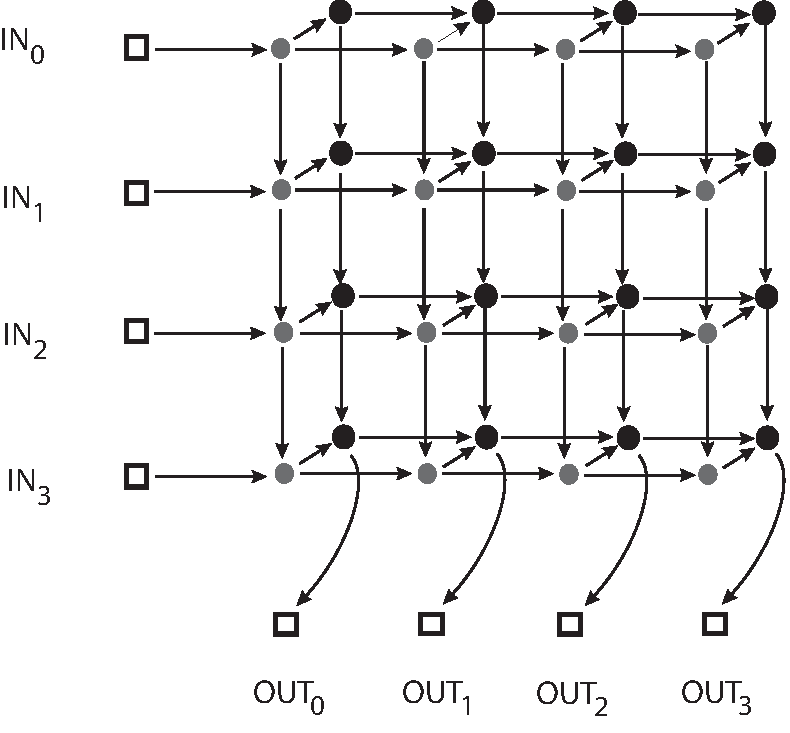
\includegraphics[width=3in,clip]{2-layer-grid.pdf}
\end{center}

In general, an $n$-input 2-layer-grid has two layers of switches, with
each layer connected like an $n$-input grid.  There is also an edge from
each switch in the first layer to the corresponding switch in the second
layer.  The inputs of the 2-layer-grid enter the left side of the first
layer, and the $n$ outputs leave the bottom of the second layer.

\bparts

\ppart[2] \; What is the latency of an $n$-input 2-layer-grid?
\brule{0.5in} \solution[\vspace{.2in}]{$2n+1$}


\ppart[4] \; For any given input-output permutation, there is a way to route
packets that achieves congestion 1.  Describe how to route the packets in 
this way.

\solution[\newpage]{To route a packet from input $i$ to output $j$, use
  the path from input $i$ to the right along row $i$ of the input layer
  until column $j$.  Then take the edge to the corresponding switch in
  column $j$ of the output layer, and continue the path downward along
  column $j$ in the output layer to output $j$.  Now each packet moves to
  the right in its own row of the input layer and down in its own column
  in the output layer, and so packets never cross.  That is, congestion is
  1.}


\eparts
\end{problem}

%%%%%%%%%%%%%%%%%%%%%%%%%%%%%%%%%%%%%%%%%%%%%%%%%%%%%%%%%%%%%%%%%%%%%%%%%%%%%%%%%%%%%%%%%%%%%%%%%%%%%%%%%%%%%%%%%%%%%%%%%%%%%%%%%%%%%%%%%%%%%%%%%%%%%%%%%%%%%%
%%%%%%%%%%%%%%%%%%%%%%%%%%%%%%%%%%%%%%%%%%%%%%%%%%%%%%%%%%%%%%%%%%%%%%%%%%%%%%%
%%%%%%%%%%%%%%%%%%%%%%%%%%%%%%%%%%%%%%%%%%%%%%%%%
% By Spyros
% Equivalence relations/equivalence classes
% From fall08 ps6old.tex first problem (parts a and b)
%
\begin{problem}{15}
In this problem we study some properties of relations. Recall that a relation $R \subseteq X \times Y$ is a set of pairs $(x,y)$.

\bparts 
\ppart{5} A function $F \subseteq X \times Y$ is a relation with the extra property that if $(x,y) \in F$ and $(x, y') \in F$, then $y = y'$. Let $Z = \{0, 1, 2, \ldots, p-1\}$. Consider the set $S$ of all pairs $(x,y) \in Z \times Z$ for which $x = y^2 \bmod p$. Prove or disprove: $S$ is a function.

\solution{$S$ is not a function. To see this, observe that $(1, 1)$ and $(1, p-1)$ both occur in $S$, since $1 \equiv 1^2 \bmod p$ and $$  1 \bmod p \equiv (-1)^2 \bmod p \equiv (p-1)^2 \bmod p.$$} 

Recall that a special type of relation is an equivalence relation, that is, a relation that is reflexive, symmetric, and transitive. For each of the following, either prove that it is an equivalence relation and state its equivalence classes, or give an example of why it is not an equivalence relation.

\ppart{5} $R:= \{(x, y) \in \{0,1\}^n \times \{0,1\}^n \mid \Delta(x,y) \leq 1\}$, where $\Delta(x,y)$ denotes the {\it Hamming distance} of $x$ and $y$, that is, the number of coordinates which differ. For instance, the strings $000$ and $010$ have Hamming distance $1$ since they differ on the second coordinate, and the strings $011$ and $110$ have Hamming distance $2$ since they differ on the first and last coordinates.

\solution{$R$ is not an equivalence relation. For $b \in \{0,1\}$, we use the notation $b^i$ to denote $i$ consecutive $b$s. Let $x = 0^n$, $y = 10^{n-1}$, and $z=1^20^{n-2}$. Then $\Delta(x,y) = 1$ and $\Delta(y, z) = 1$, but $\Delta(x,y) = 2$, so $R$ is not transitive.}

\eparts
\end{problem}



\end{document}




